\chapter{Methodology}
\label{ch:Methodology}
This chapter outlines the technical methodology adopted in the development of the system, covering both low-level design and software implementation. The approach prioritizes performance, privacy, and modularity, leveraging hardware accelerators where possible and maintaining efficient control over data flow and execution.


%----------------------
\section{Application Design - Modules}
\label{sec:ApplicationDesign-Modules}
%----------------------

This section provides an overview of the internal architecture and design principles behind the TLDR desktop application. The application is built with the goal of providing a fast, private, and efficient interface for question-answering and summarization tasks over a user-defined corpus of documents. To achieve this, the design incorporates several performance-aware and hardware-conscious modules, especially tailored for Apple’s M1/M2 architecture.

The TLDR system is structured into modular components, each responsible for a specific functionality in the information processing pipeline. These include embedding generation, context retrieval, vector storage, prompt construction, and output generation via a language model. The workflow between these modules is coordinated to support seamless execution, low latency, and high responsiveness, all while maintaining data privacy by running entirely on-device.


%----------------------
\subsection{Modules Overview}
\label{subsec:modules_overview}
%----------------------
The TLDR application follows a modular architecture where different components are responsible for distinct tasks in the RAG (Retrieval-Augmented Generation) pipeline. Figure~\ref{fig:tldr_modules} illustrates the overall design and the control flow between the modules.

\begin{figure}[H]
    \centering
    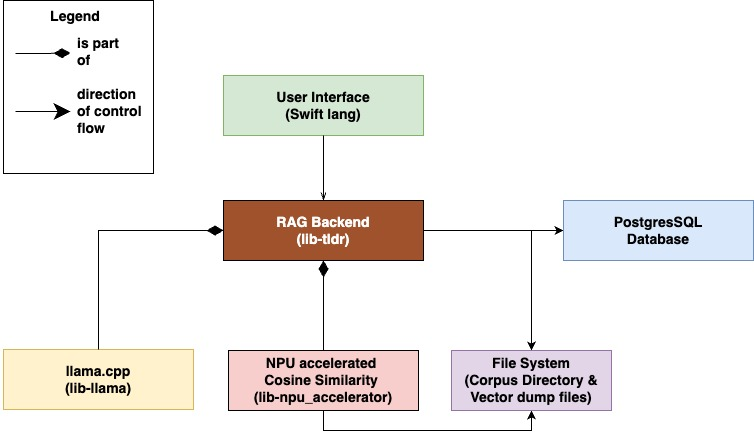
\includegraphics[width=1.0\linewidth]{images/tldr-app-modules.jpg}
    \caption{Modules of TLDR application}
    \label{fig:tldr_modules}
\end{figure}

\begin{itemize}
    \item \textbf{User Interface (Swift):} This module provides the graphical frontend for the user. Developed using Swift, it allows users to input queries, view summaries, and interact with the document corpus. All user commands are forwarded to the backend for processing.

    \item \textbf{RAG Backend (lib-tldr):} This is the core orchestrator of the application. It manages the full pipeline, including handling user queries, initiating vector search, performing retrieval, and forwarding context to the language model. It communicates with all supporting modules such as the database, vector search engine, and file system.

    \item \textbf{PostgreSQL Database:} Stores metadata and document indexing information. It ensures efficient retrieval and persistence of preprocessed documents and vector references.

    \item \textbf{File System (Corpus Directory and Vector Dump Files):} Contains the raw document corpus and their corresponding vector dump files. These vectors are accessed using memory-mapped I/O for performance and low memory overhead.


    \item \textbf{NPU Accelerated Cosine Similarity (lib-npu\_accelerator):} Implements hardware-accelerated cosine similarity using Apple's Neural Processing Unit (ANE). The backend invokes this module for fast and parallelizable similarity computation.

    \item \textbf{llama.cpp (lib-llama):} This module is responsible for language generation. Once the RAG backend compiles the context, it is passed to the llama.cpp engine for final response generation.
\end{itemize}


%----------------------
\subsection{File System: Corpus Directory and Vectordump Files}
\label{subsec:FSandVectordump_files}
%----------------------
Vector dump files are binary data structures designed for efficient storage of document embeddings. For each input document, a corresponding vector dump file is created. Each such file contains embedding vectors generated from text chunks along with their corresponding MD5 hashes. This format enables fast similarity search and content verification in document retrieval systems.

%----------------------
\subsubsection{File Structure}
\label{subsec:Vectordump_FileStructure}
%----------------------
The vector dump file follows a sequential binary layout consisting of three main components: a metadata header, followed by embedding data, and finally hash data. This structure allows for efficient random access to embeddings while maintaining data integrity through hash verification. Hash is also further used for fetching the corresponding text chunk after similar vectors are obtained for a query.

   \begin{figure}[H]
    \centering
    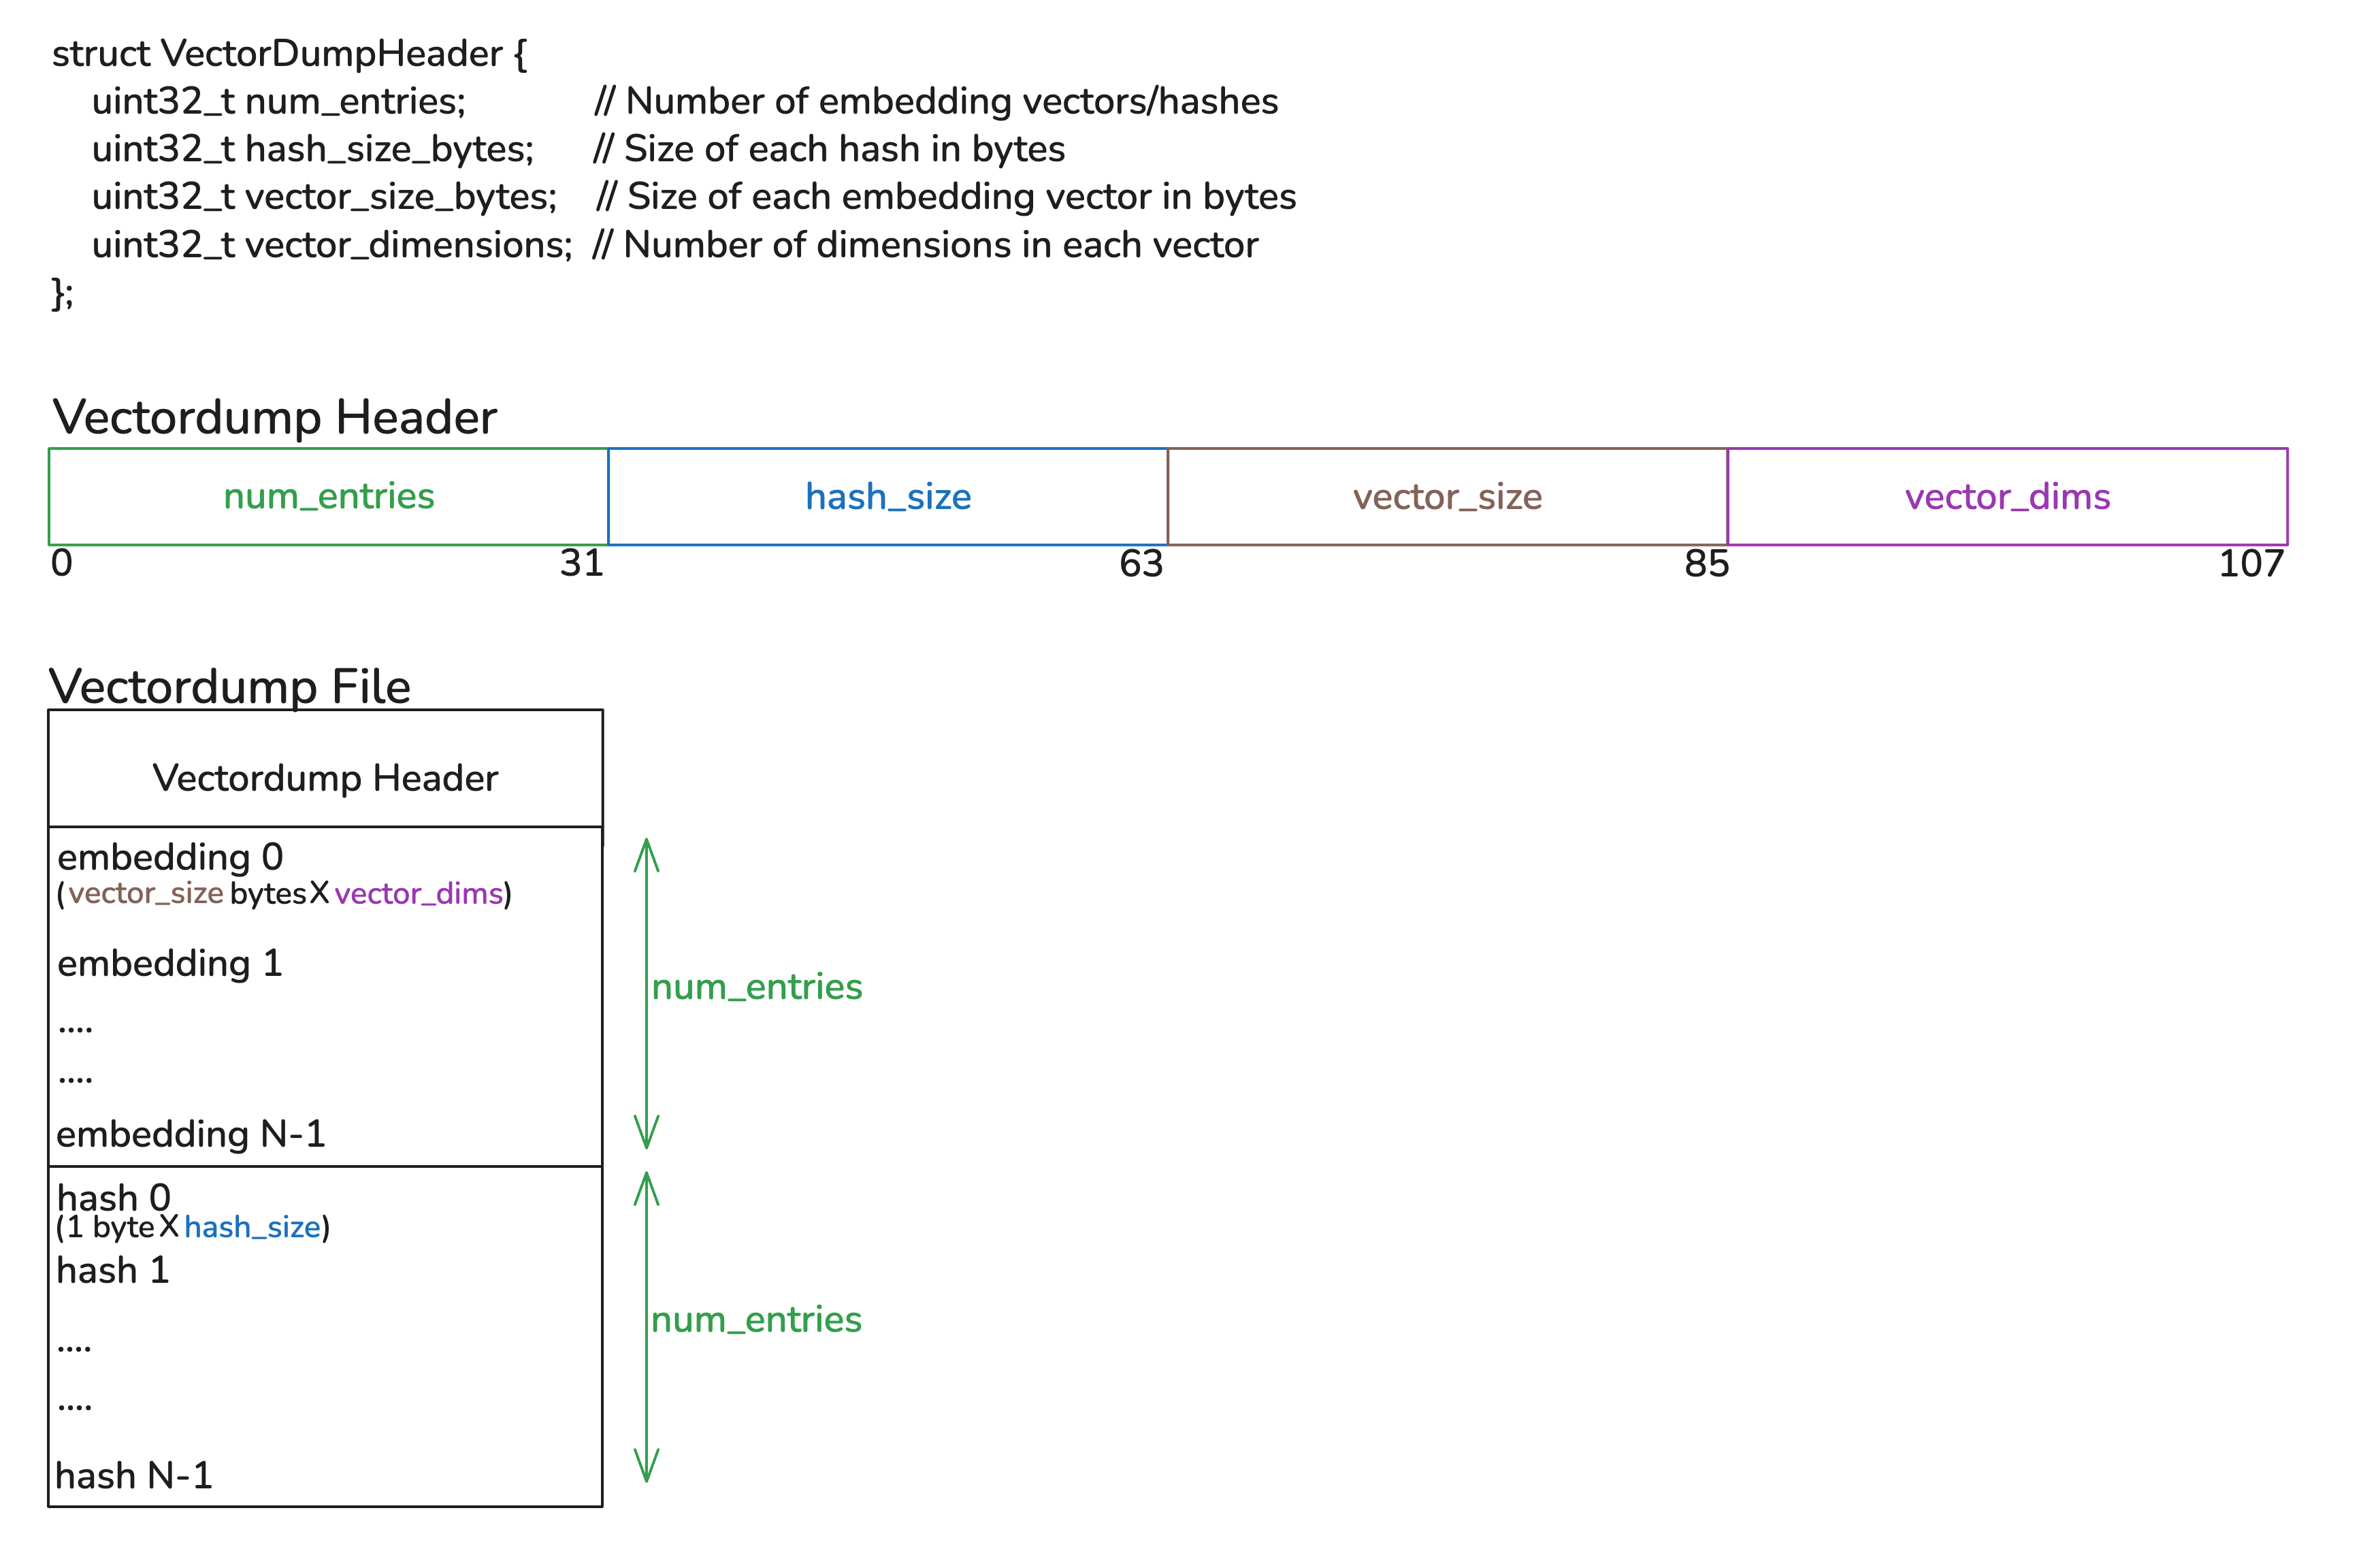
\includegraphics[width=1.0\linewidth]{images/VectorDumpFiles.png}
    \caption{Vector dump file structure}
    \label{fig:vectordumpfilestructure}
\end{figure}

%----------------------
\subsubsection{Header}
\label{subsec:Vectordump_Header}
%----------------------
In order to process the vector dump file, the header is first read and the necessary information is obtained regarding the data layout in the file. The information is arranged in the layout as illustrated in Figure~\ref{fig:vectordumpfilestructure}. The elements are as follows:
\begin{itemize}
    \item \texttt{num\_entries} - Total number of embedding/hash pairs stored in the file
    \item \texttt{hash\_size\_bytes} - Size of each MD5 hash in bytes (always 16 for standard MD5)
    \item \texttt{vector\_size\_bytes} - Total byte size of each embedding vector
    \item \texttt{vector\_dimensions} - Number of floating-point dimensions per embedding vector
\end{itemize}

The header is read by pointing the $VectorDumpHeader$ struct to the memory location of the loaded file. This helps obtain the  necessary information required to access the data sections of the file.

%----------------------
\subsubsection{Data Sections}
\label{subsec:Vectordump_DataSections}
%----------------------
Once the header section is loaded, the data obtained is then used for calculating the memory locations of the embedding and hash arrays.
Pointers are used to access these locations to simulate the structure of an array on top of raw binary data read into the memory. This approach is simple and efficient and prevents needless memory allocations and data copies.

\textbf{Embeddings:} Contains $N$ consecutive embedding vectors, where $N$ = \texttt{num\_entries}. Each vector occupies \texttt{vector\_size\_bytes} and represents a \texttt{vector\_dimensions}-dimensional embedding, typically stored as 32-bit floating-point values.

\textbf{Hashes:} Contains $N$ consecutive MD5 hash values, each exactly 16 bytes. However, the smallest unit of storage is of $uint64_t$ type, i.e., units of 2 bytes. Hence, a 16 byte MD5 hash would have a hash size of 8. The hash at index $i$ corresponds to the MD5 digest of the original text chunk used to generate \texttt{embedding[i]}.


%----------------------
\subsubsection{Data Relationship}
\label{subsec:Vectordump_DataRelationship}
%----------------------

The file maintains strict positional correspondence: for any index $i \in [0, N-1]$, \texttt{embedding[i]} and \texttt{hash[i]} represent the same document chunk. This one-to-one mapping enables efficient lookup operations and integrity verification during retrieval.

The data is used as follows:
\begin{enumerate}[label=\arabic*.]
\item Load the first half of the file in memory using \textbf{mmap} and perform cosine similarity search.
    \item Obtain index of the top $K$ relevant vectors from Cosine similarity module.
    \item Fetch the hash values at the obtained indices.
    \item Query the database for text chunks associated with the hash values.
\end{enumerate}
    
This design allows for prioritized access to necessary data and its direct usage for cosine similarity search with no further processing or data manipulations, allowing for an efficient search through the entire corpus.




User Interface RAG Backend  PostgreSQL Database NPU Accelerated Cosine Similarity  {llama.cpp
%----------------------
\subsection{File System: Corpus Directory and Vectordump Files}
\label{subsec:FSandVectordump_files}
%----------------------


%----------------------
\subsection{File System: Corpus Directory and Vectordump Files}
\label{subsec:FSandVectordump_files}
%----------------------



%----------------------
\section{Application Design - Workflow Overview}
\label{subsec:TldrWorkflowOverview}
%----------------------

\begin{figure}[H]
    \centering
    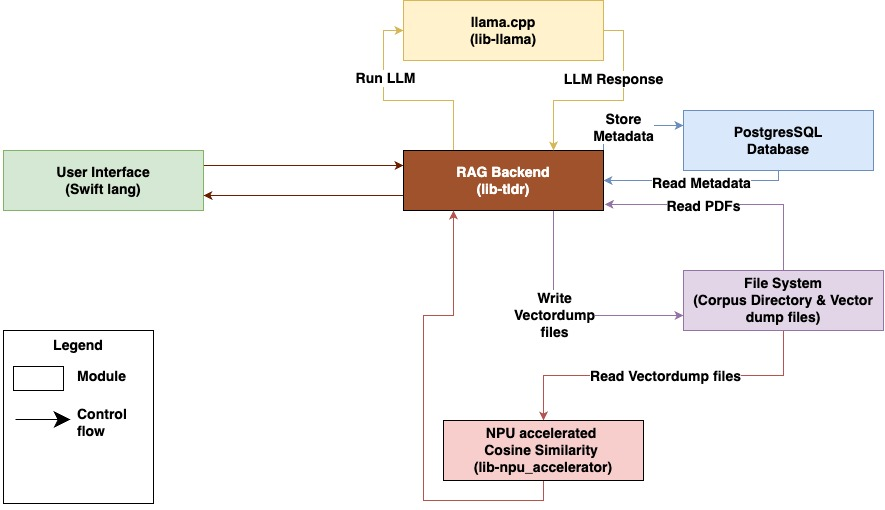
\includegraphics[width=1.0\linewidth]{images/tldr-app-module-interactions.jpg}
    \caption{RAG Output evaluation metrics ~\cite{cardenas2023rag}}
    \label{fig:autoregressive_decoding}
\end{figure}


Figure~\ref{fig:tldr_workflow} illustrates the end-to-end workflow of the TLDR application. It is divided into three primary phases: system initialization, document corpus embedding, and query-based retrieval-augmented generation (RAG).

\subsubsection{System Initialization}

\begin{figure}[H]
    \centering
    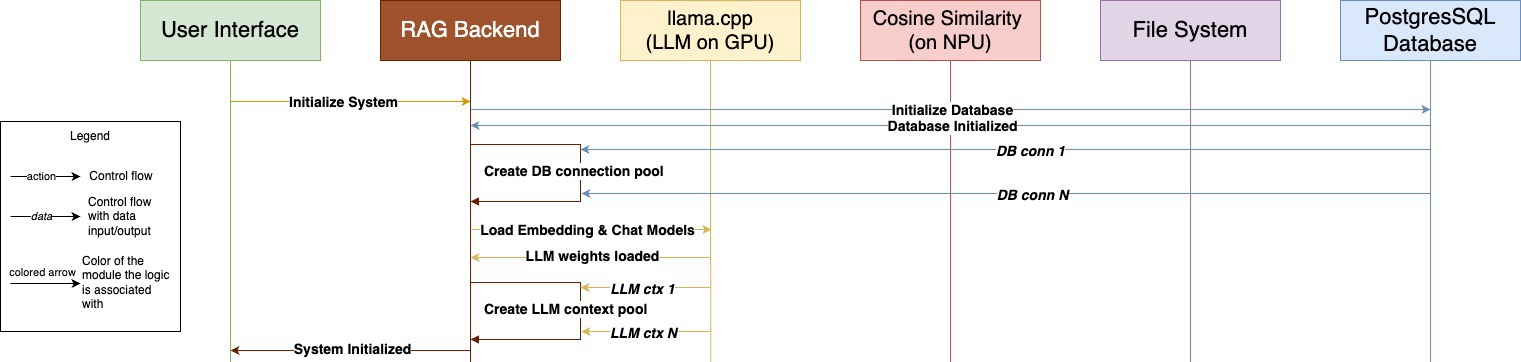
\includegraphics[width=1.0\linewidth]{images/tldr-app-worklfow-pt1.jpg}
    \caption{RAG Output evaluation metrics ~\cite{cardenas2023rag}}
    \label{fig:autoregressive_decoding}
\end{figure}


The initialization phase sets up the backend infrastructure and prepares the application for use. This includes:

\begin{itemize}
    \item The user launches the application, triggering the backend.
    \item The \textbf{RAG Backend} initializes a connection pool to the \textbf{PostgreSQL Database}.
    \item The LLM weights and context pools are loaded via \texttt{llama.cpp}, enabling multi-threaded inference.
    \item Cosine similarity routines are prepared via the \textbf{NPU accelerator} module.
    \item System status is communicated back to the \textbf{User Interface}, indicating readiness.
\end{itemize}

\subsubsection{Corpus Embedding}

\begin{figure}[H]
    \centering
    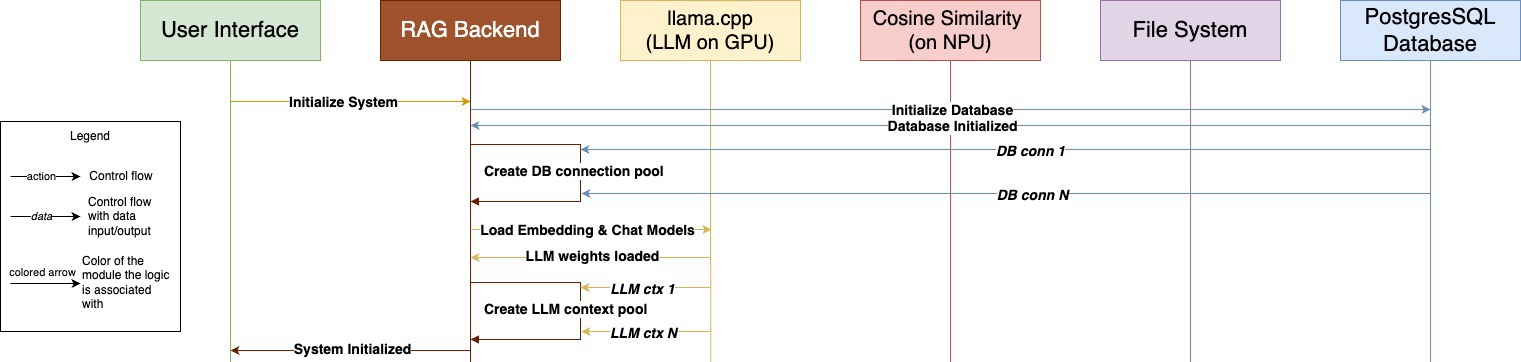
\includegraphics[width=1.0\linewidth]{images/tldr-app-worklfow-pt1.jpg}
    \caption{RAG Output evaluation metrics ~\cite{cardenas2023rag}}
    \label{fig:autoregressive_decoding}
\end{figure}

When a user specifies a directory to embed:

\begin{itemize}
    \item The \textbf{RAG Backend} scans the specified directory for documents using the File System.
    \item Each document is loaded, chunked, and converted to embeddings using a pre-defined embedder.
    \item Embeddings, text chunks, and associated metadata are inserted into the \textbf{PostgreSQL Database}.
    \item In parallel, the backend also writes a vector dump file to the \textbf{File System}, which stores the hash of each vector for quick access.
\end{itemize}

This dual-storage mechanism (DB + mmap vector cache) allows fast retrieval during inference while maintaining queryable metadata.

\subsubsection{Query Execution via RAG}

\begin{figure}[H]
    \centering
    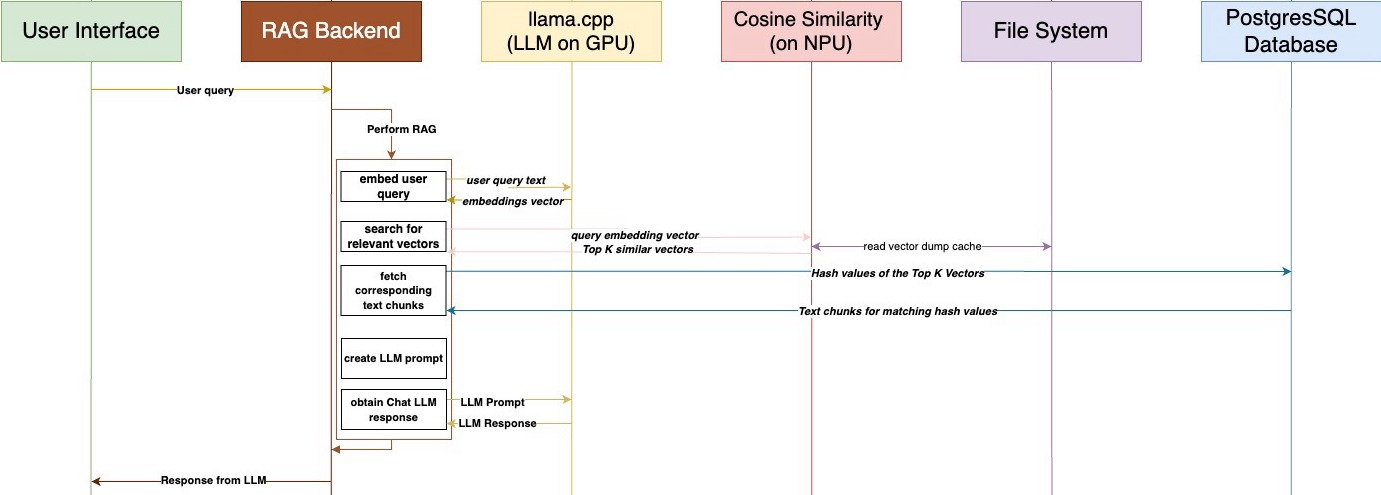
\includegraphics[width=1.0\linewidth]{images/tldr-app-worklfow-pt3.jpg}
    \caption{RAG Output evaluation metrics ~\cite{cardenas2023rag}}
    \label{fig:autoregressive_decoding}
\end{figure}

Once the corpus is embedded, the user may input a query. The following steps are executed:

\begin{itemize}
    \item The user query is embedded using the same embedding model.
    \item The embedded query vector is sent to the \textbf{Cosine Similarity} module running on the NPU.
    \item A top-$k$ similarity search is performed against memory-mapped vector files using the NPU, returning hash values of the best matches.
    \item These hashes are used to retrieve the corresponding text chunks from the \textbf{PostgreSQL Database}.
    \item A prompt is constructed and sent to the \textbf{LLM} via \texttt{llama.cpp}.
    \item The generated response is sent back to the \textbf{User Interface}.
\end{itemize}

This phase exemplifies the retrieval-augmented generation paradigm, grounded entirely in the user’s local corpus and executed with optimized hardware utilization.





%----------------------
\section{III. Application Implementation}
\label{sec:III.ApplicationImplementation}
%----------------------
